\documentclass[twoside]{article}

% We add packages, macros here:
%!TEX root =  lec-template.tex
\usepackage{lmodern}
\usepackage[english]{babel}
\usepackage{latexsym}
\usepackage{amsmath}
\usepackage{mathrsfs}
\usepackage{amssymb}
\usepackage{mathtools}
\usepackage[inline,shortlabels]{enumitem} % we prefer enumitem because of its margin adjustment caps
\usepackage{bm}
\usepackage{datetime}
\usepackage[table,xcdraw]{xcolor}
\usepackage{accents}
\usepackage{tikz}
\usepackage{listings}
\usepackage{mdframed}
\usepackage{pgfplots}
\usepackage{pgfplotstable}
\usepackage[boxed]{algorithm}
\usepackage{algpseudocode}
\usepackage{dsfont}
\usepackage{color}
\usepackage{colortbl}
\usepackage{pifont}
\usepackage[bf,font=small,singlelinecheck=off]{caption}
\usepackage{microtype} % improved spacing between words for easier reading
\usepackage{float}
\usepackage{xfrac} % sfrac
\usepackage{xspace}

\linespread{1.1}


\usepackage[textsize=tiny]{todonotes}
\makeatletter
\renewcommand{\todo}[2][]{\@todo[#1]{#2}}
\makeatother

\setlength{\marginparwidth}{10ex}
\newcommand{\todoc}[2][]{\todo[size=\scriptsize,color=blue!20!white,#1]{Csaba: #2}}
\newcommand{\todoj}[2][]{\todo[size=\scriptsize,color=red!20!white,#1]{Jincheng: #2}}

\usepackage{hyperref}
\hypersetup{
    unicode=false,          % non-Latin characters in Acrobat�s bookmarks
    pdftoolbar=true,        % show Acrobat�s toolbar?
    pdfmenubar=true,        % show Acrobat�s menu?
    pdffitwindow=false,     % window fit to page when opened
    pdfstartview={FitH},    % fits the width of the page to the window
    pdftitle={},    % title
    pdfauthor={},     % author
    pdfsubject={Theory, Machine Learning, Lectures},   % subject of the document
    pdfcreator={},   % creator of the document
    pdfproducer={}, % producer of the document
    pdfkeywords={theory} {machine learning} {lecture notes} {CMPUT 654} {Fall 2023}, % list of keywords
    pdfnewwindow=true,      % links in new window
    colorlinks=true,       % false: boxed links; true: colored links
    linkcolor=blue,          % color of internal links (change box color with linkbordercolor)
    citecolor=blue,        % color of links to bibliography
    filecolor=magenta,      % color of file links
    urlcolor=cyan           % color of external links
}
\usepackage{amsthm}
\usepackage{times}
\usepackage{natbib}
\usepackage{nicefrac}
\usepackage{wrapfig}
\usepackage[capitalize]{cleveref}
\usepackage[nottoc,numbib]{tocbibind}

%\usepackage[bmargin=0.75in]{geometry}
\usepackage[margin=1.1in]{geometry}
\usepackage[normalem]{ulem}


%%%%%%%%%%%%%%%%%%%%%%%%%%%%%%%%
% HYPHENATION
%%%%%%%%%%%%%%%%%%%%%%%%%%%%%%%%

\pretolerance=5000
\tolerance=9000
\emergencystretch=0pt
\righthyphenmin=4
\lefthyphenmin=4


\bibliographystyle{plainnat}

\newcommand{\E}{\mathbb{E}}
\newcommand{\EE}[1]{\E[#1]}
\newcommand{\PP}{\mathbb{P}}
\newcommand{\Prob}[1]{\mathbb{P}(#1)}
\newcommand{\one}[1]{\mathbb{I}\{#1\}}
\newcommand{\Supp}{\operatorname{supp}}
\newcommand{\ip}[1]{\langle #1 \rangle}
\newcommand{\bip}[1]{\left\langle #1 \right\rangle}
\newcommand{\norm}[1]{\|#1\|}
\newcommand{\R}{\mathbb{R}}
\newcommand{\N}{\mathbb{N}}
\newcommand{\cA}{\mathcal{A}}
\newcommand{\cB}{\mathcal{B}}
\newcommand{\cC}{\mathcal{C}}
\newcommand{\cD}{\mathcal{D}}
\newcommand{\cE}{\mathcal{E}}
\newcommand{\cF}{\mathcal{F}}
\newcommand{\cG}{\mathcal{G}}
\newcommand{\cH}{\mathcal{H}}
\newcommand{\cK}{\mathcal{K}}
\newcommand{\cL}{\mathcal{L}}
\newcommand{\cN}{\mathcal{N}}
\newcommand{\cP}{\mathcal{P}}
\newcommand{\cQ}{\mathcal{Q}}
\newcommand{\cR}{\mathcal{R}}
\newcommand{\cS}{\mathcal{S}}
\newcommand{\sA}{\mathscr A}

\newcommand{\cM}{\mathcal{M}}
\newcommand{\cX}{\mathcal{X}}
\newcommand{\cY}{\mathcal{Y}}
\newcommand{\NN}{\mathbb{N}}
\newcommand{\RR}{\mathbb{R}}
\newcommand{\VV}[1]{\mathbb{V}[#1]}

\newcommand{\epsapp}{\epsilon}
\newcommand{\epssub}{\delta}

\DeclareMathOperator{\Range}{range}
\newcommand{\rows}{\operatorname{rows}}

\renewcommand{\epsilon}{\varepsilon}
\newcommand{\ceil}[1]{\left\lceil {#1} \right\rceil}
\newcommand{\floor}[1]{\left\lfloor {#1} \right\rfloor}
\newcommand{\ones}{\mathbf{1}}
\newcommand{\zeros}{\mathbf{0}}
\DeclareMathOperator*{\argmin}{arg\ min}
\DeclareMathOperator*{\argmax}{arg\ max}


\def\rvzero{{\mathbf{0}}}
\def\rvone{{\mathbf{1}}}

\def\identiymatrix{\mathbf{Id}}

\newcommand{\softmax}{\mathrm{softmax}}
\newcommand{\KL}{D_{\mathrm{KL}}}

% Graph
\def\gA{{\mathcal{A}}}
\def\gB{{\mathcal{B}}}
\def\gC{{\mathcal{C}}}
\def\gD{{\mathcal{D}}}
\def\gE{{\mathcal{E}}}
\def\gF{{\mathcal{F}}}
\def\gG{{\mathcal{G}}}
\def\gH{{\mathcal{H}}}
\def\gI{{\mathcal{I}}}
\def\gJ{{\mathcal{J}}}
\def\gK{{\mathcal{K}}}
\def\gL{{\mathcal{L}}}
\def\gM{{\mathcal{M}}}
\def\gN{{\mathcal{N}}}
\def\gO{{\mathcal{O}}}
\def\gP{{\mathcal{P}}}
\def\gQ{{\mathcal{Q}}}
\def\gR{{\mathcal{R}}}
\def\gS{{\mathcal{S}}}
\def\gT{{\mathcal{T}}}
\def\gU{{\mathcal{U}}}
\def\gV{{\mathcal{V}}}
\def\gW{{\mathcal{W}}}
\def\gX{{\mathcal{X}}}
\def\gY{{\mathcal{Y}}}
\def\gZ{{\mathcal{Z}}}

% Sets
\def\sA{{\mathbb{A}}}
\def\sB{{\mathbb{B}}}
\def\sC{{\mathbb{C}}}
\def\sD{{\mathbb{D}}}
% Don't use a set called E, because this would be the same as our symbol
% for expectation.
\def\sE{{\mathbb{E}}}
\def\sF{{\mathbb{F}}}
\def\sG{{\mathbb{G}}}
\def\sH{{\mathbb{H}}}
\def\sI{{\mathbb{I}}}
\def\sJ{{\mathbb{J}}}
\def\sK{{\mathbb{K}}}
\def\sL{{\mathbb{L}}}
\def\sM{{\mathbb{M}}}
\def\sN{{\mathbb{N}}}
\def\sO{{\mathbb{O}}}
\def\sP{{\mathbb{P}}}
\def\sQ{{\mathbb{Q}}}
\def\sR{{\mathbb{R}}}
\def\sS{{\mathbb{S}}}
\def\sT{{\mathbb{T}}}
\def\sU{{\mathbb{U}}}
\def\sV{{\mathbb{V}}}
\def\sW{{\mathbb{W}}}
\def\sX{{\mathbb{X}}}
\def\sY{{\mathbb{Y}}}
\def\sZ{{\mathbb{Z}}}

\newcommand{\dimE}{\mathrm{dim}_{\mathcal{E}}}
\DeclareMathOperator{\diam}{diam}


%%
%% ADD PACKAGES here:
%%
%
%\usepackage{amsmath,amsfonts,graphicx}
%
%
% The following commands set up the lecnum (lecture number)
% counter and make various numbering schemes work relative
% to the lecture number.
%

\newcounter{lecnum}
\renewcommand{\thepage}{\thelecnum-\arabic{page}}
\renewcommand{\thesection}{\thelecnum.\arabic{section}}
\renewcommand{\theequation}{\thelecnum.\arabic{equation}}
\renewcommand{\thefigure}{\thelecnum.\arabic{figure}}
\renewcommand{\thetable}{\thelecnum.\arabic{table}}


%
% The following macro is used to generate the header.
%
\newcommand{\lecture}[4]{
   \pagestyle{myheadings}
   \thispagestyle{plain}
   \newpage
   \setcounter{lecnum}{#1}
   \setcounter{page}{1}
   \noindent
   \begin{center}
   \framebox{
      \vbox{\vspace{2mm}
    \hbox to 6.28in { {\bf CMPUT 654 Fa 23: Theoretical Foundations of Machine Learning \hfill Fall 2023} }
       \vspace{4mm}
       \hbox to 6.28in { {\Large \hfill Lecture #1: #2  \hfill} }
       \vspace{2mm}
       \hbox to 6.28in { {\it Lecturer: #3 \hfill Scribes: #4} }
      \vspace{2mm}}
   }
   \end{center}
   \markboth{Lecture #1: #2}{Lecture #1: #2}

   \noindent {\bf Note}: {\it 
   \LaTeX\  template courtesy of UC Berkeley EECS dept. (\href{https://inst.eecs.berkeley.edu/~cs294-8/sp03/Materials/}{link} to directory)
   }

   \noindent {\bf Disclaimer}: {\it These notes have \underline{\textbf{not}} been subjected to the
   usual scrutiny reserved for formal publications. They may be
   distributed outside this class only with the permission of the
   Instructor.} \vspace*{4mm}
}
%
% Convention for citations is authors' initials followed by the year.
% For example, to cite a paper by Leighton and Maggs you would type
% \cite{LM89}, and to cite a paper by Strassen you would type \cite{S69}.
%%%%%%%%% (To avoid bibliography problems, for now we redefine the \cite command.)
%%%%%%%%% Also commands that create a suitable format for the reference list.
%%%%%%%%\renewcommand{\cite}[1]{[#1]}
%%%%%%%%\def\beginrefs{\begin{list}%
%%%%%%%%        {[\arabic{equation}]}{\usecounter{equation}
%%%%%%%%         \setlength{\leftmargin}{2.0truecm}\setlength{\labelsep}{0.4truecm}%
%%%%%%%%         \setlength{\labelwidth}{1.6truecm}}}
%%%%%%%%\def\endrefs{\end{list}}
%%%%%%%%\def\bibentry#1{\item[\hbox{[#1]}]}

%Use this command for a figure; it puts a figure in wherever you want it.
%usage: \fig{NUMBER}{SPACE-IN-INCHES}{CAPTION}
\newcommand{\fig}[3]{
			\vspace{#2}
			\begin{center}
			Figure \thelecnum.#1:~#3
			\end{center}
	}
% Use these for theorems, lemmas, proofs, etc.

%!TEX root =  lec-template.tex
%%%%%%%%%%%%%%%%%%%%%%%%%%%%%%%%
% THEOREMS
%%%%%%%%%%%%%%%%%%%%%%%%%%%%%%%%
\theoremstyle{plain}
\newtheorem{theorem}{Theorem}[lecnum]
\newtheorem{claim}[theorem]{Claim}
\newtheorem{proposition}[theorem]{Proposition}
\newtheorem{lemma}[theorem]{Lemma}
\newtheorem{corollary}[theorem]{Corollary}
\newtheorem{example}[theorem]{Example}
\theoremstyle{definition}
\newtheorem{definition}[theorem]{Definition}
\newtheorem{assumption}[theorem]{Assumption}
\newtheorem{remark}[theorem]{Remark}
\newtheorem{exercise}[theorem]{Exercise}
\theoremstyle{remark}


%\newtheorem{theorem}{Theorem}[lecnum]
%\newtheorem{lemma}[theorem]{Lemma}
%\newtheorem{proposition}[theorem]{Proposition}
%\newtheorem{claim}[theorem]{Claim}
%\newtheorem{corollary}[theorem]{Corollary}
%\newtheorem{definition}[theorem]{Definition}
%\newenvironment{proof}{{\bf Proof:}}{\hfill\rule{2mm}{2mm}}

% **** IF YOU WANT TO DEFINE ADDITIONAL MACROS FOR YOURSELF, PUT THEM HERE:

\newcommand{\set}[1]{\left\{#1\right\}}
\newcommand{\I}{\mathbb{I}}
\newcommand{\cW}{\mathcal{W}}


\begin{document}
%FILL IN THE RIGHT INFO.
%\lecture{**LECTURE-NUMBER**}{**DATE**}{**LECTURER**}{**SCRIBE**}
\lecture{22}{November 28}{Csaba Szepesv\'ari}{Kushagra Chandak}
%\footnotetext{These notes are partially based on those of Nigel Mansell.}

% **** YOUR NOTES GO HERE:

% Some general latex examples and examples making use of the
% macros follow.  
%**** IN GENERAL, BE BRIEF. LONG SCRIBE NOTES, NO MATTER HOW WELL WRITTEN,
%**** ARE NEVER READ BY ANYBODY.

\section{Outline}
\begin{itemize}[-]
    \item Introduction to neural networks.
    \item Function approximation.
    \item Depth vs width in neural networks.
\end{itemize}

\section{Neural Networks}
A two-layered (one hidden and one output layer) fully connected neural network with $m$ units in the hidden layer is a map $f: \R^d \to \R$ given by
\[
    f_w(x) = \sum_{i=1}^m u_i h(\theta_i^\top x + b_i) \,,
\]
where $h:\R \to \R$ is the activation function, $x \in \R^d$ is the input vector, $\theta_i \in \R^d$ is the weight vector, $b_i \in \R$ is the bias/threshold, $u_i \in \R$ is the weight to the output, and $w = (\theta, u, b) \in \R^{m(d+2)}$ are the parameters.



\subsection{Function Approximation with Neural Networks}
Let $\cF_m^{(h)} = \set{f_w : w \in \cW_m}$, where $\cW_m = \R^{m(d+2)}$, be the two-layered neural network function class with $m$ hidden units and activation function $h$. The next theorem shows that $f \in \cF_m$ is a universal approximator.

In this section, we will see how well we can approximate functions of different kinds with neural networks.
\begin{theorem}[Leshno, 1993]
    Let $h: \R \to \R$ be such that $h \notin \R[x]$ (not a polynomial). Let $K \subset \R^d$ be compact. Then $\cF_m^{(h)}|_K = \set{f|_K : f \in \cF_m^{(h)}}$ is dense in $C(K)$.
\end{theorem}

To state the next result, let us introduce a set of functions
\[
    \Gamma_r = \set{f:\R^d \to R: \exists \tilde f : \R^d \to C \text{ s.t. } f(x) = \int e^{i\omega^\top x} \tilde f(\omega) d\omega, \, \forall x \in B_r}\,,
\]
where $B_r = \set{x^d : \norm{x}_2 \le r}$ is a ball of radius $r$. The function $\tilde f$ is the Fourier transform of $f$ up to constant factors. We have a complexity/smoothness measure/coefficient for $f \in \Gamma_r$ (assuming there exists a unique $\tilde f$ for $f$):
\[
    C(f) = \int \norm{\omega}_2 |\tilde f(\omega)| d\omega \,.
\]
The quantity $C(f)$ roughly measures the ``energy" of $f$ at high frequency. Thus, $f$ is smooth if $C(f)$ is small. With $C(f)$ in hand, we state our next result:   

\begin{theorem}[Barron, 1993]\label{thm:barrons}
    Let $h: \R \to \R$ be a measurable bounded function such that $\lim_{z \to -\infty} h(z) = 0$ and $\lim_{z \to \infty} h(z) = 1$. Let $f \in \Gamma_r$ such that $C(f) < \infty$ and $\mu \in \cM_1(B_r)$. Then for all $m \ge 1$
    \[
        \inf_{w \in \cW_m} \norm{f - f(0) - f_w}_{L_2(\mu)} \le \frac{(2 r C(f))^2}{m}\,.
    \]
\end{theorem}
\begin{remark}
    Note that the above result is independent of $d$. When we approximate a smooth function with polynomial, we get a rate of roughly $(1/m)^{s/d}$, where $s$ is the number of continuous derivative of the target function $f$. So the above result does not tell us that for any smooth function, the approximation error goes down with $1/m$ rate. But functions with finite $C(f)$ creates a subset of smooth functions for which we get the $1/m$ rate (see \cref{fig:barrons-thm}).    
\end{remark}

\begin{remark}
    Some of the common choices of the activation function are sigmoid ($h(z) = 1/(1+e^{-z})$) and ReLU ($h(z) = \max(0,z)$). Note that while sigmoid satisfies the condition of \cref{thm:barrons}, ReLU does not. However, for ReLU, we can write $s(z) = h(z) - h(z-1)$ such that $s$ satisfies the condition.
\end{remark}

\begin{figure}{h}
    \centering
    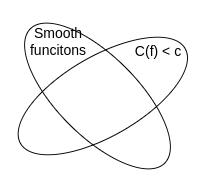
\includegraphics[height=3cm, width=4cm]{figures/barrons-thm.png}
    \caption{Barron's theorem (\cref{thm:barrons}) does not hold for all smooth functions but only a ``slice".}
    \label{fig:barrons-thm}
\end{figure}


\paragraph{Does depth in neurals networks give some advantage?}
For the next result, let $d=1$ and the activation function is ReLU. We also index the neural network class with number of layers:
\[
    \cF_{k, m} = \set{ f:[0,1]\to\R : \text{ $f$ can be implemented by a NN with $\le k$ layers and $\le m$ hidden units}} \,. 
\]

\begin{theorem}[Telgarsky, 2016]\label{thm:deep-shallow-nn}
    Let $k \ge 3$. Then 
    \[
        \sup_{f \in \cF_{2k^2, 2}} \inf_{g \in \cF_{k, 2^{k-2}}} \norm{f-g}_\infty \ge \frac{1}{16}\,.
    \]
\end{theorem}
\emph{Proof intuition. }
The proof is done by constructing a function $f_k$ which is difficult to approximate using shallow networks. Let $f_0(x) = \max(0, \min(2x, 2(1-x)))$ on $[0,1]$. Note that $f_0(x)$ can be implemented by a 2 layer neural network with $m=2$, $\theta_1 = 2$, $\theta_2 = -4$, $b_1 = 0$, and $b_2 = -0.5$ so that 
\[
    f_0(x) = 2 \max(0,x) - 4\max(0, x-0.5) = w_1 h(x) + w_2 h(x-0.5) \,.
\]
Let $f_k(x) = f_0(f_{k-1}(x))$ with $k \ge 1$. Then $f_k(x)$ can be represented by a $2k$ layer neural network with 2 units in each hidden layer. \cref{fig:f0} shows $f_k$ for $k=0,1,2$. 

\begin{figure}[h]
    \centering

 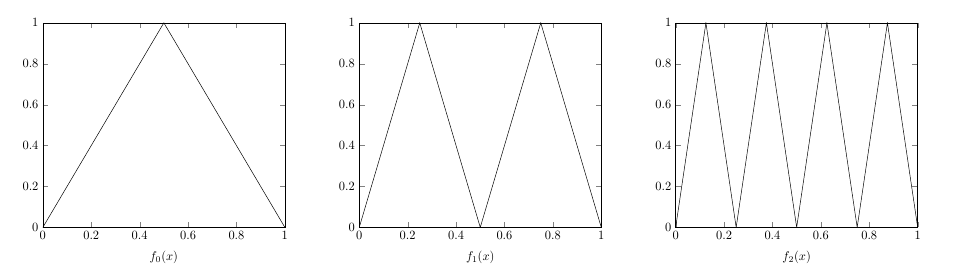
\includegraphics[width=\linewidth]{figures/nn-telgarsky.png}
    \caption{$f_k(x)$ for $k=0, 1, 2$.}
    \label{fig:f0}
\end{figure}

\begin{definition}[Crossing Number]
    The crossing number of a function $f:[0,1] \to [0,1]$ is the number of segments in the graph on which $f$ is above the line $y=\frac12$.
\end{definition}
Combining the below two claims gives us the result. 
\begin{claim}
    For every measurable $g:[0,1] \to [0,1]$ such that $C(g) < 2^{k-1}$, $\norm{f_k - g}_{L_1} \ge \frac{1}{16}$.
\end{claim}

\begin{claim}
We have that
\[
        \max\set{ C(g) : g \in \cF_{l,m} } \le 2(2m)^l \,.
\]
\end{claim}
 
\end{document}
